% \iffalse meta-comment
%
% Copyright (C) 2004-2012 by Robert Marik <marik@mendelu.cz>
% ----------------------------------------------------------
% 
% This file may be distributed and/or modified under the
% conditions of the LaTeX Project Public License, either version 1.2
% of this license or (at your option) any later version.
% The latest version of this license is in:
%
%    http://www.latex-project.org/lppl.txt
%
% and version 1.2 or later is part of all distributions of LaTeX 
% version 1999/12/01 or later.
%
% \fi
%
% \iffalse
%<*driver>
\ProvidesFile{fancytooltips.dtx}
%</driver>
%<package>\NeedsTeXFormat{LaTeX2e}[1999/12/01]
%<package>\ProvidesPackage{fancytooltips}
%<*package>
    [2012/06/12 v1.12 fancytooltips.dtx  file]
%</package>
%
%<*driver>
\documentclass{ltxdoc}
\EnableCrossrefs         
\CodelineIndex
\RecordChanges
\OnlyDescription
\usepackage{xcolor,graphicx,listings}
\usepackage[filename=tip,mouseover,movetips,fg]{fancytooltips}
\buttontipwidth=2cm
\buttontipheight=2cm
\begin{document}
\color{black}
  \DocInput{fancytooltips.dtx}
\end{document}
%</driver>
% \fi
%
% \CheckSum{1186}
%
% \CharacterTable {Upper-case
% \A\B\C\D\E\F\G\H\I\J\K\L\M\N\O\P\Q\R\S\T\U\V\W\X\Y\Z Lower-case
% \a\b\c\d\e\f\g\h\i\j\k\l\m\n\o\p\q\r\s\t\u\v\w\x\y\z Digits
% \0\1\2\3\4\5\6\7\8\9 Exclamation \!  Double quote \" Hash (number)
% \# Dollar \$ Percent \% Ampersand \& Acute accent \' Left paren \(
% Right paren \) Asterisk \* Plus \+ Comma \, Minus \- Point \.
% Solidus \/ Colon \: Semicolon \; Less than \< Equals \= Greater than
% \> Question mark \?
% Commercial at \@     Left bracket  \[     Backslash     \\
% Right bracket \] Circumflex \^ Underscore \_ Grave accent \` Left
% brace \{ Vertical bar \| Right brace \} Tilde \~}
%
%
% \changes{v1.0}{2007/02/15}{Initial version}
%
% \changes{v1.1}{2007/02/20}{Clener code, better documentation, fix
%   for bug with delayinterval macro, support for dvips and Distiller
%   users.}  
%
% \changes{v1.2}{2007/03/01}{Better support for dvips users, buttons
%   for icons are created automatically using eso-pic package and have
%   the name "ikona.pagenumber", new option \texttt{movetips}, tooltip
%   appears on the current page only and, as a consequence, animations
%   are faster.}
%
% \changes{v1.3}{2007/05/08}{Fixed bug which appears in dvips route.
%   Improved documentation -- added a note about the required version
%   of eforms.sty}
%
% \changes{v1.4}{2009/04/29}{Added support for presentations (like
%   \texttt{pause} command for texpower).}
%
% \changes{v1.5}{2009/05/05}{Handling number of pages via aux file
%   (fixes some problems issued by previous modification and page
%   break near tooltip).}
%
% \changes{v1.6}{2010/04/10}{Added options \texttt{debug},
%   \texttt{active} and \texttt{inactive}, added an example with
%   automatic previews for equations and floats. Added handling of
%   this.dirty and app.focusRect. Changed the name of the file with
%   tooltips. Added starred version of \texttt{tooltip} command.}
%
% \changes{v1.7}{2010/05/20}{Added options \texttt{blur} and
%   \texttt{fg}, cleaned some command names}
%
% \changes{v1.8}{2010/06/10}{Added hook do insert stuff on each page.}
%
% \changes{v1.9}{2011/12/04}{Changed expansion in the new |\ref|
% command provided by |FancyHook| macro (see |fancy-preview|
% facility).}
%
% \changes{v1.10}{2012/05/09}{New script preview-latex. New options
% |previewall| and |nosoap|.}
%
% \changes{v1.11}{2012/05/11}{Fixed bug related to bad position if
% |fg| option is used and \texttt{evensidemargin} is different from
% \texttt{oddsidemargin}.}
%
% \changes{v1.12}{2012/06/12}{Documentation updated. New option
% |tooltipmark|.}
%
% \GetFileInfo{fancytooltips.dtx}
%
% \DoNotIndex{\newcommand,\newenvironment}
% 
%
% \title{The \textsf{fancytooltips} package, the \textsf{fancy-preview} script\thanks{This document
%     corresponds to \textsf{fancytooltips}~\fileversion, dated
%     \filedate.} \thanks{Supported by grants 18/2006, 99/2008 and 131/2010
%     of Higher
%     Education Development Fund (FRV\v S) }} \author{Robert Ma\v r\'\i k \\
%   \texttt{marik@mendelu.cz}}
%
% \maketitle
%
% \setcounter{tocdepth}{2}\tableofcontents\rightskip=0em plus 0.2em\sloppy
% \section{Introduction}
%
% The \LaTeX{} package |fancytooltips| allows to insert tooltips into
% PDF documents -- a popup windows appears if the mouse hovers or
% clicks particular area. You can use plain text as well as
% mathematics, pictures and animations in your tooltips. The PDF
% viewer must interpret Javascripts to make the tooltips work. This is
% currently true only for (free) Abobe Reader and (commercial) Adobe
% Acrobat. There are two ways how to produce the PDF file. The
% simplest way is to use |pdflatex|. Another option is |latex| +
% |dvips| + AdobeDistiller\footnote{not free |ps2pdf|} + Adobe
% Acrobat\footnote{not free Adobe Reader.}.
%
% \color{black}Here you can test two tooltips: \tooltip{Einstein's
% formula}{1} and simple \tooltipanim{animation}{2}{7} (numbers from 1
% to 6). For more examples how the presentation may look like see the
% |examples| subdirectory. We also provide a Perl script
% |fancy-preview| which allows to extract equations, theorems and
% related parts of text into separate PDF file and insert tooltips
% after each |\ref|, |\eqref| and |\cite| command automatically. For
% more information see Figure \ref{fig:1} and demos (scientific
% papers, presentations, tests) at
% \url{http://user.mendelu.cz/marik/fancy-preview}.
%
% Related \LaTeX{} packages are |cooltooltips|, |pdfcomment| (smaller
% size of the resulting PDF, but restricted to plain text), |ocgtools|
% (works with layers, only |pdflatex| is supported) and Acro\TeX{}
% (works with layers, only |latex| + |dvips| + Adobe Distiller + Adobe
% Acrobat are supported). All these ``similar'' packages allow to
% write the text for the tooltips inside the main document. In
% contrast to this approach, |fancytooltips| package makes use of an
% external file. This allow to use graphics or mathematical
% expressions in the tooltips.
%
% The package requires |eforms.sty| and |insdljs.sty| packages, which
% are part of AcroTeX bundle
% (\url{http://www.math.uakron.edu/~dpstory/webeq.html}).
%
% \section{Usage of \texttt{fancytooltips.sty}}
% \subsection{Small technical background}
% 
% \begin{itemize}
% \item The pages from the external PDF file with tootlips are
%   inserted as icons at hidden buttons into the resulting
%   PDF. 
% \item If you insert tooltip, the current page is covered by an
%   invisible transparent button which spans across the whole page
%   (the information about the pages with tooltips is stored in |aux|
%   file and hence we have to run \LaTeX{} \textit{three times}). The
%   button has an associated JavaScript action to close all tooltips
%   (i.e. make itself and other related buttons hidden).
% \item Another button which reveals tooltip is created. This button
%   is transparent, covers the text typeset by \TeX{} and allows to
%   activate a JavaScript. This JavaScript takes the picture required,
%   puts this picture as icon to the button which covers the
%   corresponding page and makes this button visible.
% \item Each page has an associated action which closes all tooltips
%   when the page is opened.
% \end{itemize}
% 
% \subsection{The file with tooltips} 
% The file with tooltips is an ordinary PDF file, one tooltip per
% page. Tooltips should be in the top right corner at the page, in a
% \textit{box with nontransparent background} and the rest of the page
% should be transparent. If you consider to use |movetips| option
% which causes the tooltip appear near the mouse cursor instead of in
% the top right corner (see below), then every page should have the
% dimensions equal to the dimensions of the colored box with
% tooltip\footnote{Look at the files \texttt{tooltipy.tex} and
% \texttt{tooltipy.pdf} from |examples| subdirectory for a simple
% example how to meet this condition under pdf\LaTeX. You may also use
% ordinary \LaTeX{} class, set \texttt{\textbackslash pagestyle\{empty\}} and crop the boundary.}. You can
% call the tooltips by their page numbers, but for better comfort we
% also provide simple cross referencing mechanism. If the pdf file is
% created by \LaTeX, \DescribeMacro{\keytip} you can define keywords
% to refer to the pages using |\keytip| command.  Simply put
% |\usepackage[createtips]{fancytooltips}| into preamble and write
% \texttt{\string\keytip}\marg{foo} in document. This writes
% information about keyword \meta{foo} and the pagenumber into file
% |\jobname.tips|. See
% \url{http://user.mendelu.cz/marik/fancytooltips} for some tooltip
% templates.
%
% \subsection{The file with presentation}
% In the file with presentation, the user is responsible to
% \begin{itemize}
% \item input either |color| or |xcolor| package in the
%   preamble
% \item \LaTeX{} the file two times (we write some macros into |aux|
%   file) or three times (if option |fg| is used).
% \end{itemize}
% You may use the following options to set the necessary information
% and change the default behavior of the package.
%
% \def\iitem#1{\item[{\color{blue!50!black}\texttt{#1}}]} 
% \begin{description}\sloppy\rightskip 0 pt plus 1 em
%   \iitem{filename} To input the tooltips from file \meta{foo.pdf}
%   call the package with |filename| option:
%   |\usepackage[filename=foo]{fancytooltips}|. This option is
%   required if compiled with |pdflatex|.
%
% \iitem{movetips} By default, tooltip appears in the
% top right corner of the page (use View--PageLayout-Single Page in
% your Adobe Reader, please). If the option |movetips| is used, then
% tooltip appears close to the mouse pointer. More precisely, tooltip
% appears with left down corner at the mouse position, if there is
% enough place. If not, tooltip appears with right down corner at the
% mouse position. Finally, the tooltip is shifted down to fit the
% page, if necessary\footnote{This option works in this way if every
%   page of the file with tooltips has dimensions of the box with
%   tooltip.  See the \texttt{examples} subdirectory.}.
%
%
%   \iitem{mouseover} If you use |mouseover| option,
%   then tooltip appears if you move the mouse pointer to the active
%   area (no clicking is necessary).
%
%   \iitem{inactive} This option makes the package
%   inactive.
%
%   \iitem{active} This option forces the package
%   active even if |inactive| option is loaded.
%
%   \iitem{blur} The rest of the page is blurred, when showing
%   tooltip. Use either |\usepackage[blur]{fancytooltips}| or
%   |\usepackage[blur=number]{fancytooltips}|, where |number| is
%   a number between 0 and 1. (Note that we use transparent package
%   and hence this could have an influence on the colors of the
%   document and could make your PDF less portable.) This option is
%   allowed in pdf\LaTeX{} mode only. If this options brakes colors
%   only on the page which include tooltips, you may want to use
%   option |fixcolor| to fix it.
%
%   \iitem{fixcolor} See |blur| option.
%
%   \iitem{debug} Prints two alerts reporting success or problems when
%   opening PDF file in Adobe Acrobat (Adobe Reader).  Use this option
%   to find possible source of problems. See also the Section
%   \ref{sec:tr} in this manual.  
%
%   \iitem{noextratext} No mark is appended at the end of the link
%   which opens tooltips (see help for |\tooltip|).
%
%   \iitem{nosoap} A single space is used to occupy the space for
%   button produced by |\tooltip*| command instead of blue soap. As a
%   result, the button produced by |\tooltip*| works as usual, but it
%   is invisible. This is sometimes convenient for the user, since the
%   mark does not disturb the text. However, the author has to
%   instruct the user, that the hidden buttons follow links from
%   cross references.
%
%   \iitem {fg} The button for displaying pictures is placed on
%   background and the buttons which activate tooltips are placed
%   immediately in the text by default. With |fg| option all these
%   buttons are placed into foreground after the page is completed. We
%   use |\pdfsavepos| command and keep track of the position for
%   buttons in aux file and hence this option works in pdf\LaTeX\ only
%   and the file needs more compilations. This option does not do
%   anything in dvi mode now (despite the fact that pdf\LaTeX\
%   provides the feature also for dvi mode), but this could be changed
%   if someone requests this feature. Use this option for example, if
%   you use frame around hyperlinks or buttons and form fields in your
%   PDF (like tests produced by Acro\TeX).
%
%   \iitem{preview} Redefines |\ref|, |\eqref| and |\cite| commands to
%   work with tooltips extracted by |fancy-preview|, see Section
%   \ref{sec:fancy-preview} and demo files in |example/fancy-preview|
%   directory. The tooltip is inserted only if the target of the
%   reference is on different PDF page as the tooltip. This option is
%   suitable for presentations where the whole PDF page is
%   visible. Replaces former |\FancyHook| command.
%
%   \iitem{previewall} Like |preview| but shows tooltip also if the
%   target is on the same page. Suitable for enhanced versions of
%   papers written on A4 page.
%
%   \def\aaa#1{#1\hbox
%   {\smash{\raisebox{0.4em}{\includegraphics[width=0.7em]%
%   {fancytipmark#1.pdf}}}}} \iitem{tooltipmark} Allows to change the
%   tooltipmark to some predefined styles, values are \aaa1, \aaa2,
%   \aaa3 and \aaa4. Note that you can change the mark to whatever
%   different by redefining |\TooltipExtratext| command. Work only in
%   pdflatex mode. 
%
% \end{description}
% 
% \DescribeMacro{\tooltip} The user can put the tooltip into her or
% his presentation using the command
% \texttt{\string\tooltip}{\marg{stuff}\marg{keyword-or-pagenumber}}
% where \meta{stuff} is the printed text in \meta{tooltipcolor} color
% and \meta{keyword-or-pagenumber} is either the pagenumber of the
% tooltip in the external file or the keyword defined by |\keytip|
% command and stored in |\TooltipFilename.tips| file, where
% |\TooltipFilename| is set automatically from the |filename| option.
% \DescribeMacro{\TooltipExtratext} The printed text \meta{stuff} is
% followed by |\TooltipExtratext| command. The default value is small
% blue soap, as you have seen in the second paragraph of this
% documentation. There is a |noextratext| option which defines
% |\TooltipExtratext| to be empty. \DescribeMacro{noextratext option}
% If \marg{keyword-or-pagenumber} is not recognized as valid keyword
% for tooltips, it is supposed to be pagenumber.
%
% The text \marg{stuff} is inserted in |\hbox| by
% |\tooltip|. \DescribeMacro{\tooltip*}With starred version of the
% |\tooltip| macro the text \marg{stuff} is not inserted into the box
% and the active button dos not cover the text \marg{stuff}, but
% covers the mark produced by |\TooltipExtratext|.
% 
% \DescribeMacro{\tooltipanim}\DescribeMacro{\tooltipanim*} The user
% can put a series (animation) of tooltips into the presentation by
% using \texttt{\string\tooltipanim}\marg{stuff}\marg{start}\marg{end}
% command, where \meta{start} and \meta{end} are keywords defined by
% |\keytip| command or page numbers.  \DescribeMacro{\delayinterval}
% The delay between two frames is |\delayinterval| milliseconds. The
% default value is 200, you can change it by command
% |\def\delayinterval{100}|. There is also starred version which works
% similarly like |\tooltip*| command.
%
% \DescribeMacro{\TooltipRefmark} Extra text added to |\ref|, |\eqref|
% and |\cite| commands with previews, see Section
% \ref{sec:fancy-preview}. The default value is the same as for
% |\TooltipExtratext|.
%
% \subsubsection{Changes for dvips users}
% Dvips users also have to prepare tooltips into PDF file, not eps as
% usual. But we have to insert these tooltips in Adobe Acrobat Pro
% program. If you use Acrobat Pro version 8.1 and later, install the
% file \texttt{aeb.js} from AcroTeX eDucation bundle as described in
% the documentation to AcroTeX.\footnote{If you do not install
%   \texttt{aeb.js} properly, you can still create your presentation,
%   but you have to import the |fdf| file manually, see the section
%   Troubleshooting and known problems.}
%
% Since \LaTeX{} is not capable to find the number of pages in
% external PDF file with tooltips, \DescribeMacro{dvips}dvips users have to specify option
% |dvips| in |fancytooltips| package.  \DescribeMacro{pages} You have
% to use also a |pages| option with the number of pages in the PDF
% file with tooltips, if you use dvips route. You have to call the
% package by
% something like this:\\
% |\usepackage[dvips,filename=tooltipy,pages=27]{fancytooltips}|
% 
% You have to |latex| (two times) and |dvips| your file first.  This
% produces |filename.ps| and |Tooltipsdljs.fdf| files. Distill the
% |filename.ps| file into |filename.pdf| and open this file by Adobe
% Acrobat Professional -- this imports macros from |Tooltipsdljs.fdf|
% file. In Acrobat's JavaScript console (open by |Crtl+J|) run (using
% |Ctrl+Enter|) the command |ImportTooltips();| which is defined for
% the document. This command inserts invisible buttons on the first
% page, imports icons (the file with icons specified as
% \meta{filename} parameter when loading fancytooltips must be in
% working directory). You should see a message ``\texttt{importing
%   pictures}'' and the command returns 1 when finished. Then
% \textbf{save the file} (you can use the same name). If the command
% |ImportTooltips();| fails, you either have not the PDF file with
% tooltips in current directory, or the PDF file does not contain
% JavaScripts. In the latter case insert document level JavaScripts
% manually as described in the Section \ref{sec:tr}.
%
% \section{Tootlips at
% references: \texttt{fancy-preview}} \label{sec:fancy-preview} 
% \subsection{Basic usage}
% There is a Perl script |fancy-preview| which can be used to extract
% text from bibliography items, numbered equations, numbered theorems,
% lemmas, etc, put this text into separate PDF file and add this text
% as tooltips to the corresponding |\ref|, |\eqref| and |\cite|
% commands. Reading the resulting file may look like on Figure
% \ref{fig:1}.
% \begin{figure}
%   \centering
%\fbox{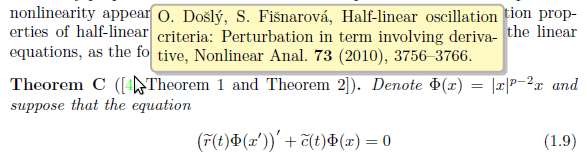
\includegraphics[width=0.95\textwidth]{cite.png}}
%   \caption{\texttt{fancy-preview}}
%   \label{fig:1}
% \end{figure}
% 
%
% The script |fancy-preview| has been tested with Texlive2011 on both
% Linux and MS Windows. To run this script you need working Perl
% installation (usually present on Linux workstations, on MS Windows
% you may need to install Perl from
% \url{http://www.activestate.com/activeperl}) and |Config::IniFiles|
% module\footnote{Package |libconfig-inifiles-perl| on Ubuntu Linux,
% |cpan Config::IniFiles| or |ppm install Config::Inifiles| on MS
% Windows. Alternatively you can run |ppm| without any parameters to
% invoke the GUI.})
%
%   To compile your document |file.tex| do the following
%   \begin{itemize}
%   \item Put |\usepackage{hyperref}| into the preamble of your document
%     (if not already loaded).
%   \item If you write references in |thebibliography| environment, put
%     empty line after each |\bibitem| command (including the last item
%     in |thebibliography|).
%   \item Run |fancy-preview file|. After several compilations you
%     should get the PDF file |file.pdf|.
%   \end{itemize}
%   The default work-flow is the following.  The file is compiled with
%   |pdflatex| to get correct numbers of equations and in the first
%   pass of |preview.sty| we extract displayed equations (but the
%   numbers are thrown away). After this we crop the PDF file by using
%   |pdfcrop| program (an alternate program can be specified as
%   optional parameter). Then we extract numbered environments
%   (theorem, Theorem, lemma, corollary, definition, figure, table)
%   using the second pass and crop the PDF file again. After this we
%   merge all equations, theorems etc which are marked with |\label|
%   command. The PDF file with extracted parts of the text is the used
%   as source of toltips in final compilations.
%
% Many things can be customized. The following options are
% available.
% \begin{description}
%   \iitem{pdfcrop} You may specify an alternative batch file to crop
%   boundary of PDF file. Default is |pdfcrop|. The command line for
%   an alternative program to crop PDF file is supposed to be the
%   following: |programname input.pdf output.pdf|. Using optimal
%   program to PDF file may be much fasater and may produce
%   significantly smaller files. \iitem{tooltips} You may combine
%   the tooltips extracted by |fancy-preview| with ``ordinary hand
%   made tooltips''. Simply call |fancytooltips| in the main document
%   by |\usepackage[inactive]{fancytooltips}| in your document and
%   specify the file with tooltips in the command line of the
%   |fancy-preview| or in the |ini| file. You may also compile your
%   file by |pdflatex| and get ``normal'' PDF output (the compilation
%   is way faster). \iitem{fancy\underline{ }options} Options passed
%   |fancytooltips| in final compilations. Default is
%   |previewall,nosoap|. Options |mouseover| and |movetips| are added
%   automaticaly.\iitem{ini\underline{ }file}Specifices the |ini| file
%   with configuration, see the next subsection.
% \end{description}
% \subsection{Configuration from ini files}
% Other customization can be done via |ini| files. The script looks
% for customizations in the file specified by |ini_file| command line
% parameter. If this parameterer is not used, the script looks for
% customization in two default locations: |~/.fancy-preview.ini| and
% in |./fancy-preview.ini| (both files are used if both exist). You
% can use |~/.fancy-preview.ini| for customizations related to all
% your projects and |./fancy-preview.ini| for projects in the current
% directory. The options from the file
% |./fancy-preview.ini| override |~/.fancy-preview.ini| and the
% options from command line override options from
% |./fancy-preview.ini|. The format is described at
% \url{http://search.cpan.org/~shlomif/Config-IniFiles-2.75/lib/Config/IniFiles.pm}.
%
% The parameters are divided into two sections, |[main]| and |[latex]|.
% In section |[main]| of |ini| file you can set parameters |pdfcrop|,
% |tooltips| and |fancy_options|. 
% 
% In the section |[latex]| if the initialization file you can
% customize the compilation by \LaTeX. Here you can set parameters
% |environments| and |snarfenvironments| to set the environments which
% will be extracted. The default values are
% |environments=Theorem,theorem,lemma,corollary,definition| and
% |snarfenvironments=figure|.
%
% The material from |tex| file is extracted in three passes. These
% passes are denoted by |a|, |b| and |c|. If
% \texttt{\string\label}\marg{foo} appears in the text which is marked
% for extraction, then the corresponding
% \texttt{\string\newlabel}\marg{foo} command is written to the |aux|
% file and \meta{foo} is supposed to be the name of the keyword
% corresponding to the PDF page with the text.
%
% If a referenced material appears in more passes, then the priority
% is set in the variable |$latex{'pass_order'}| and can be customized
% in the ini file in |[latex]| section as |pass_order| parameter. The
% default value is |pass_order=acb|, i.e.  |c| overrides |b| and |a|
% overrides |c|.
%
% As a typical example consider equation with label |\label{eq}| in
% numbered theorem with label |\label{th}|. The equation is extracted
% in pass |a| (displayed equation) and in pass |b| (the whole
% theorem). The corresponding |\newlabel{eq}| command appers in two
% |aux| files -- from passes |a| and |b|. The first one corresponds to
% the PDF page with equation, the latter to the PDF page with whole
% theorem. Since |a| overrides |b|, then |\ref{eq}| and |\eqref{eq}|
% commands show the number of the equation followed by the tooltip
% with equation only. Further |\ref{th}| shows number of the theorem
% followed by the tooltip with the whole theorem. If you set |pass_order=ba|, then both |\ref{eq}| and |\ref{th}| are followed by the
% same tooltip.
%
% The following options are available\footnote{These
% options are used as keywords in a hash variable \texttt{latex}, i.e. for
% default value of \texttt{param} parameter search the file \texttt{fancy-preview}
% for \texttt{\$latex\{'param'\}}.}.
%\begin{itemize}
%  \iitem {a} Defines commands for the first pass. It
%  inserts |preview.sty| command which extracts displayed
%  mathematics. Also resets |\tagform@| and |\@eqnnum| to skip
%  printing of equation numbers.
%  \iitem {a\underline{ }extra} Defines material which is appended to |a|
%
%  \iitem {b} Defines commands fot the second pass. In this \LaTeX{}
%  run are (by default) floating figures and theorem-like environments
%  extracted. Inserts |preview.sty|. At the runtime,
%  |\PreviewEnvironment[{[]}]{env}| and
%  |\PreviewSnarfEnvironment[{[]}]{env}| for each |env| in comma
%  separated list from |environments| and |snafenvironments| is added,
%  respectively.
%  \iitem {b\underline{ }extra} Defines material which is appended to |b|
%
% \iitem{environments} See |b| option. 
%
% \iitem{snarfenvironments} See |b| option. Default value is |figure|.
%
% \iitem {c} If empty (default value), then the third pass is
% skipped. Otherwise, you may activate |preview.sty| similarly like in
% |b| (for a template see the source code and the default setting of
% |$latex{'b'}|) and extract environments and commands according to
% your interest. A possible application is to extract |minipage|
% environments, if there are two or more figures inserted in
% |minipage| environments into one |figure| environment.
%
% \iitem{pass\underline{ }order} Sets priority, which pass is supposed
% to produce the output for a |\label| which is extracted more times
% than once, see the previous paragraphs for explanation and example.
%
% \iitem{preview\underline{ }bibitem} Redefines |\bibtem| command. The
% material between |\bibitem| and |\par| is wrapped to the width of
% |0.75\textwidth| and extracted.
%
% \iitem{preview\underline{ }biblatex} Similarly like
% |preview_bibitem| but works with |biblatex|.
%
% \iitem{ini} Inserted at the begin of each |pdflatex| run.
%
% \iitem{tooltips\underline{ }envelope\underline{ }preamble} Used in
% preamble. Defines command |\tooltipwraper|. This command wraps the
% tooltips. Default is to use |tikz| to put everything into a yellow
% box with rounded corners and shading. 
%
% \iitem{biblatex} Creates temporary file
% |fancy-preview-biblatex-settings.tex|. This file contains definition
% which allow |biblatex| to work with citations and tooltips and we
% input this file in final compilations. This code comes from
% |tex.stackexchange.com|.
%\end{itemize}
%
% 
%
% \subsection{Tips and tricks} 
% \begin{itemize}
% \item The program |pdfcrop| from \TeX live may produces large PDF
%   files. See the discussion at
%   \url{http://tex.stackexchange.com}\footnote{\url{http://tex.stackexchange.com/questions/42236/pdfcrop-generates-larger-file}}. The
%   smaller size can be obtained with the solution from the discussion
%   below the question, which is based on |gs| and |pdftk|. The
%   |python| script from the same discussion produces slightly larger
%   file than |pdftk|, but still much smaller than |pdfcrop| and
%   provides the fastest solution.
% \item Do not use floats in environments, which are
%   extracted. Otherwise you get an error from \LaTeX. A workaround
%   could be also to change temporarily definition of the floating
%   environment (redefine |figure| environment, for example).
% \item If you are not interested in customization via |ini| files and
%   do not want to install extra modules to your Perl installation,
%   you may delete the about twenty lines from |fancy-preview|
%   starting with |use Config::IniFiles;| up to the line
%   |read_config("./fancy-preview.ini");|
% \end{itemize}
%
% \section{Troubleshooting and known problems}\label{sec:tr}
% The source code is in Mercurial repository at
% \url{http://bitbucket.org/robert.marik/fancytooltips/}. You can also
% report problems and issues in the forum at this site. The code on
% |bitbucket.org| is considered as development version and repository
% for older versions. The last stable version is always the version
% from CTAN.
% \begin{itemize}
% \item 
%   The package works with |eforms.sty| from version
%   2006/10/03 v1.0a. You can download this or newer version from
%   \url{http://www.acrotex.net} site.
% \item If the graphics included by |\TooltipExtratext| and
%   |\TooltipRefmark| has colors with \textbf{custom opacity}, Adobe
%   Acrobat Pro sometimes renders the pictures bad. No problems of
%   this type have been observed with free Adobe Reader.
% \item For \textbf{dvips} users: In some cases the file
%   |Tooltipsdljs.fdf| is \textbf{not imported automatically}
%   (probably some setting in Adobe Acrobat or new versions of
%   |eforms.sty| and |insdljs.sty|). In this case you do not see any
%   message when using |debug| option. You have troubles of this type
%   if you see in the Javascript console (Ctrl+J) error messages like
%   ``\texttt{aebTrustedFunctions is not defined 3:Page:Open
%     CloseTooltips is not defined 1:Page:Open}''. In this case you
%   have to import the file |Tooltipsdljs.fdf| \textbf{manually from
%     ``Form'' menu} in Adobe Acrobat Pro. Then go to the JavaScript
%   console and run |ImportTooltips();| command.
% \end{itemize}
% 
% Follow the points below if you want to find the source of your
% problems.
% \begin{itemize}
% \item For dvips users it is a good idea to check that Acro\TeX{} is
%   properly installed. Do the demo files from Acro\TeX{} work for you?
% \item Try to use |debug| option, prepare the PDF file and open it in
%   Adobe Acrobat or Adobe Reader.
%   \begin{itemize}
%   \item You should see two messages when opening the file. If not,
%     the Javascript do not work in your document (are not inserted
%     properly).
%   \item Both messages should report success for pdflatex users. For
%     dvips users one of the message should report error and if you
%     run |ImportTooltips();| command in Javascript console, you should
%     see a message in Javascript console which confirms that the
%     pictures from external PDF file have been imported. If you save
%     the PDF file and open again, both messages should report
%     success.
%   \end{itemize}
% \end{itemize}
%
% \PrintChanges
% \StopEventually{}
%
% \section{Implementation}
%    \begin{macrocode}
%<*package>
\RequirePackage{graphicx}
\RequirePackage{xkeyval}
\RequirePackage{atbegshi}

\newif\if@fancytooltips@createtips\@fancytooltips@createtipsfalse
\DeclareOptionX{createtips}{\@fancytooltips@createtipstrue}

\newif\ifTooltip@usepdftex\Tooltip@usepdftextrue
\DeclareOptionX{dvips}{\Tooltip@usepdftexfalse}

\newif\if@fancytooltips@extratext\@fancytooltips@extratexttrue
\DeclareOptionX{noextratext}{\@fancytooltips@extratextfalse}

\newif\if@fancytooltips@movetips\@fancytooltips@movetipsfalse
\DeclareOptionX{movetips}{\@fancytooltips@movetipstrue}

\newif\if@fancytooltips@mouseover\@fancytooltips@mouseoverfalse
\DeclareOptionX{mouseover}{\@fancytooltips@mouseovertrue}

\newif\if@fancytooltips@inactive\@fancytooltips@inactivefalse
\DeclareOptionX{inactive}{\@fancytooltips@inactivetrue}

\newif\if@fancytooltips@active\@fancytooltips@activefalse
\DeclareOptionX{active}{\@fancytooltips@activetrue}

\newif\if@fancytooltips@fg\@fancytooltips@fgfalse
\DeclareOptionX{fg}{\@fancytooltips@fgtrue}

\DeclareOptionX{filename}{\xdef\TooltipFilename{#1}}
\DeclareOptionX{pages}{\xdef\TooltipPages{#1}}

\newif\if@fancytooltips@blur\@fancytooltips@blurfalse
\DeclareOptionX{blur}[0.4]{\@fancytooltips@blurtrue
  \xdef\fancytooltips@transparency{#1}}

\newif\if@fancytooltips@fixcolor\@fancytooltips@fixcolorfalse
\DeclareOptionX{fixcolor}{\@fancytooltips@fixcolortrue}

\newif\if@fancytooltips@preview\@fancytooltips@previewfalse
\DeclareOptionX{preview}{\@fancytooltips@previewtrue}

\newif\if@fancytooltips@previewall\@fancytooltips@previewallfalse
\DeclareOptionX{previewall}{\@fancytooltips@previewtrue\@fancytooltips@previewalltrue}

\newif\if@fancytooltips@nosoap\@fancytooltips@nosoapfalse
\DeclareOptionX{nosoap}{\@fancytooltips@nosoaptrue}

\def\@@fancytipmark{}
\DeclareOptionX{tooltipmark}{\xdef\@@fancytipmark{#1}}

\def\fancytooltipsdebugmsg{}
\DeclareOptionX{debug}{\def \fancytooltipsdebugmsg
{
if (this.getField("ikona") == null) 
  {app.alert("No buttons for placing tootlips are available. Contact the author. The file may  need more compilations.");} 
  else 
  {app.alert("Buttons for placing tooltips are available. Congratulations! Hope everything will work.");}
if (this.getField("animtiph") == null) 
  {app.alert("No hidden buttons containing tooltips available. The interactive features will not work. \n\n If you created the file by dvips, run the command ImportTooltips() in the Javascript console (Ctrl+J, write the command followed by semicolon and Ctrl+Enter).");} 
  else 
  {app.alert("Hidden buttons containing tooltips are available. Congratulations! Hope everything will work.");}
}}

\ProcessOptionsX

\if@fancytooltips@blur
\ifTooltip@usepdftex\else 
\@fancytooltips@blurfalse
\AtEndDocument{\PackageWarning{fancytooltips}
  {Blur option is incompatible with dvips. ^^J The option blur is turned off }}
\fi
\fi

\ifTooltip@usepdftex\else 
\@fancytooltips@fgfalse
\fi

\newdimen\buttontipwidth   
\newdimen\buttontipheight  
\newdimen\fancy@a
\newdimen\fancy@b
\newdimen\fancy@layerHshift\fancy@layerHshift=0pt
\newdimen\fancy@layerVshift\fancy@layerVshift=0pt
\newdimen\fancy@button@Vshift \fancy@button@Vshift=0pt
\newdimen\fancy@button@Hshift \fancy@button@Hshift=0pt
\newtoks\pos@fancy@toks

\if@fancytooltips@active\@fancytooltips@inactivefalse\fi

\if@fancytooltips@inactive
\newcommand{\tooltip}{\@ifstar\tooltip@Star\tooltip@NoStar}%
\newcommand{\tooltip@Star}[2]{#1}%
\newcommand{\tooltip@NoStar}[2]{#1}%

\newcommand{\tooltipanim}{\@ifstar\tooltipanim@Star\tooltipanim@NoStar}%
\newcommand{\tooltipanim@Star}[3]{#1}%
\newcommand{\tooltipanim@NoStar}[3]{#1}%
\def\keytip#1{}%
\def\TooltipPage#1#2{}%
\let\TooltipExtratext\relax
\let\TooltipRefmark\relax
\ifx\@ocg@makeknown\undefined
  \def\@ocg@makeknown#1#2#3{}\fi
\def\fancy@@pushButton#1#2#3#4#5#6#7#8{}
\def\fancy@@anim@pushButton#1#2#3#4#5#6#7#8#9{}

\PackageWarning{fancytooltips}{Fancytooltips inactive}%
\expandafter\endinput\fi

%    \end{macrocode}
% Each |\ref| command has associated a number and writes new label
% into aux file. If the target page for the ref is different from the
% page with this |\ref| command, the corresponding tooltip is inserted.
%    \begin{macrocode}
\newcount\fancycheckcount\fancycheckcount=0
\def\fancy@second#1#2#3#4{#2}

\def\fancypreview@refhook{%
\global\let\oldref\ref
\gdef\ref##1{\oldref{##1}\global\advance\fancycheckcount by 1\relax
\edef\templabel{fancyanchorref:\the\fancycheckcount}%
\expandafter\label\expandafter{\templabel}%
\expandafter\ifx \csname FancyToolTip@##1\endcsname\relax \else\hbox to 0 pt{%
%    \end{macrocode}
% Here we extract the page number for the label destination.
%    \begin{macrocode}
  \expandafter\ifx \csname r@##1\endcsname \relax\else
    \expandafter\let\expandafter\fancytooltip@temp@a\csname r@##1\endcsname
    \edef\fan@tempa{\expandafter\fancy@second\fancytooltip@temp@a}%
  \fi
%    \end{macrocode}
% Here we extract the page number of the |\ref| command via faked label |fancyanchorref:\the\fancycheckcount|.
%    \begin{macrocode}
  \expandafter\ifx \csname r@fancyanchorref:\the\fancycheckcount\endcsname \relax\else
    \expandafter\let\expandafter\fan@temp@w\csname r@fancyanchorref:\the\fancycheckcount\endcsname
    \edef\fan@temp@ww{\expandafter\fancy@second\fan@temp@w}%
    \fi
%    \end{macrocode}
% We print tooltip after |\ref| only if both |\label| and |\ref| commands are on different pages
%    \begin{macrocode}
\if@fancytooltips@previewall\def\fan@tempa{not a page number}\fi
\ifx\fan@tempa\fan@temp@ww\else\smash{%
  \let\TooltipExtratext\relax\tooltip{\strut\TooltipRefmark}{##1}}%
\fi
\hss}%
\fi}%
%    \end{macrocode}
% We replace the cite command. We test if natbib is loaded, if not, we redefine the command from article.cls. 
%    \begin{macrocode}
\ifx\NAT@citea@mbox\undefined
\def\@citex[##1]##2{\leavevmode
    \let\@citea\@empty
    \@cite{\@for\@citeb:=##2\do
      {\@citea\def\@citea{,\penalty\@m\ }%
        \edef\@citeb{\expandafter\@firstofone\@citeb\@empty}%
        \if@filesw\immediate\write\@auxout{\string\citation{\@citeb}}\fi
        \@ifundefined{b@\@citeb}{\hbox{\reset@font\bfseries ?}%
          \G@refundefinedtrue
          \@latex@warning
          {Citation `\@citeb' on page \thepage \space undefined}}%
        {\ifx\csname r@fancy:cite:\@citeb\endcsname\undefined \@cite@ofmt{\csname b@\@citeb\endcsname}\else\tooltip*{\@cite@ofmt{\csname b@\@citeb\endcsname}}{fancy:cite:\@citeb}\fi
        }}}{##1}}%
\else
\def\NAT@citea@mbox{%
 \@citea\mbox{\NAT@hyper@{{\citenumfont{\NAT@num}}}}\tooltip*{}{fancy:cite:\@citeb}}
\fi
}

\if@fancytooltips@nosoap
  \def\TooltipRefmark{\hbox{\ }}%
\else
  \ifTooltip@usepdftex
  \def\TooltipRefmark{\hbox {\smash{\raisebox{0.4em}{\includegraphics[width=0.7em]%
          {fancytipmark\@@fancytipmark.pdf}}}}}%
  \else
  \def\TooltipRefmark{\hbox {\smash{\raisebox{0.4em}{\includegraphics[width=0.7em]%
          {fancytipmark.eps}}}}}%
  \fi%\ifTooltip@usepdftex
\fi%\if@fancytooltips@nosoap

\if@fancytooltips@preview\AtBeginDocument{\fancypreview@refhook}\fi

\if@fancytooltips@createtips
%    \end{macrocode}
% This part (three lines) is processed if the option |createtips| is
% used. In the opposite case we process the second part, up to the end
% of the package.
%    \begin{macrocode}
\newwrite\tipfile
\immediate\openout\tipfile \jobname.tips
\def\keytip#1{\write\tipfile{\string\tooltipname{#1}{\arabic{page}}}}
\expandafter\endinput\fi
%    \end{macrocode}
% This part is processed if the option |createtips| is not used. We
% define macros which put the hidden button with the name |ikona.n| in
% the background of the page |n|, if one of the commands |\tooltip| or
% |\tooltipanim| has been used on this page. Javascripts defined by
% |\tooltip| and |\tooltipanim| commands then unhide this button and
% show the corresponding picture.
%    \begin{macrocode}

\ifx\TooltipFilename\undefined
\PackageWarning{fancytooltips}{** The filename with tooltips is not given. **}
\fi

\ifTooltip@usepdftex
\RequirePackage[pdftex]{eforms}
\def\TooltipExtratext{\hbox{\smash{\raisebox{0.4em}{\includegraphics[width=0.7em]%
        {fancytipmark\@@fancytipmark.pdf}}}}}
\else
\RequirePackage[dvips]{eforms}
\def\TooltipExtratext{\hbox{\smash{\raisebox{0.4em}{\includegraphics[width=0.7em]%
        {fancytipmark.eps}}}}}
\fi%\ifTooltip@usepdftex

\if@fancytooltips@nosoap
  \def\TooltipExtratext{\hbox{\ }}%
\fi%\if@fancytooltips@nosoap

\if@fancytooltips@extratext\else\let\TooltipExtratext\relax\fi

\AtBeginDocument{ 
\global\buttontipwidth=\paperwidth
\global\buttontipheight=\paperheight
}

\ifTooltip@usepdftex
\def\frametip@{%
  \pdfstartlink user{%
    /Subtype /Widget
    /F 6
    /T (ikona.\thepage)
    /FT /Btn
    /Ff 65536
    /H /N
    /BS << /W 1 /S /S >>
    /MK << /TP 1 /IF <</A[1.0 1.0]/SW /B>>  >>
  }%
  \vbox to \buttontipheight {\vss\hbox to \buttontipwidth{\hss}}\pdfendlink}%
\else
%    \end{macrocode}
% For dvips users we use the macros from eqxerquiz.sty package.
%    \begin{macrocode}
\def\everyeqIcon#1{\def\every@eqIcon{#1}}
\def\every@eqIcon{}
\newcommand\eqIconFTT[4][]
{%
  \push@@Button{#1}{#2}{#3}{#4}{}{\eq@setButtonProps\eq@Button@driver}%
  {\eqIconDefaults\every@ButtonField\every@eqIcon}%
}
\def\eqIconDefaults
{%
  \rawPDF{}\S{}\mkIns{/TP 1 /IF<</A[1.0 1.0]/SW/B>>}\R{0}
  \CA{}\RC{}\AC{}\BC{}\BG{}\H{B}
  \textColor{0 g}\Ff{\FfReadOnly}
}
\def\frametip@{\eqIconFTT[\BC{}\BG{}\F{\FHidden}]%
  {ikona.\thepage}{\paperwidth}{\paperheight}%
}%
\fi%\ifTooltip@usepdftex

\def\fancytooltips@one{1}
\if@fancytooltips@blur
  \RequirePackage{ocg}
  \ifx\fancytooltips@one\fancytooltips@transparency
    \def\transparent#1{}
  \else
    \RequirePackage{transparent} 
  \fi
\else
  \ifx\@ocg@makeknown\undefined
    \def\@ocg@makeknown#1#2#3{}\fi
\fi

\if@fancytooltips@fg
\else
\RequirePackage{eso-pic}
\def\frametip{%
  \expandafter\ifx \csname TooltipPage\thepage\endcsname\relax
  \else
  \setbox0=\hbox{\frametip@}%
  \hbox{\raise \dp0 \box0}
  \fi}%
\AddToShipoutPicture{\hbox to 0 pt{\frametip\hss}}
\fi

\def\fancytooltips@save@position{\pdfsavepos%
  \write\@auxout{\string\global\string \fancy@layerVshift \the\pdflastypos sp\string\relax}%
  \write\@auxout{\string\global\string \fancy@layerHshift \the\pdflastxpos sp\string\relax}%
  \global\let\fancytooltips@save@position\relax%
}

\def\fancy@beginshipout@hook{}
\AtBeginShipout{%
\TooltipPageopencloseJS
\setbox\AtBeginShipoutBox=\hbox{%    
  \hbox to 0 pt{\TooltipHidden}\global\def\TooltipHidden{}%
  \fancy@beginshipout@hook\if@fancytooltips@fixcolor\hbox to 0 pt{\resizebox{1pt}{!}{\TooltipExtratext}\hss}\fi
  \hbox to 0 pt{\box\AtBeginShipoutBox\hss}%
  \ifTooltip@usepdftex 
    \fancytooltips@save@position
    \if@fancytooltips@blur
      \expandafter\ifx \csname TooltipPage\thepage\endcsname\relax \else
      \lower\fancy@layerVshift\hbox to 0 pt{\kern-\fancy@layerHshift\relax
        \begin{ocg}{fancyOCG\thepage}{fancyOCG\thepage}{0}%
          \expandafter\transparent\expandafter{\fancytooltips@transparency}%
          \color{black}%
          \vbox to 0 pt{\vss\hbox{\vrule width \paperwidth height \paperheight}}%
        \end{ocg}\hss}%
      \fi
    \fi%\if@fancytooltips@blur
    \if@fancytooltips@fg
      \expandafter\ifx \csname TooltipPage\thepage\endcsname\relax
      \else
        \lower\fancy@layerVshift\vbox to 0 pt{\vss\hbox to 0 pt{\kern-\fancy@layerHshift\relax\hbox{\frametip@}\hss}}%
      \fi%\ifx
      \lower\fancy@layerVshift\vbox to 0 pt{\vss\hbox to 0 pt{\kern-\fancy@layerHshift\relax\hbox to 0 pt{\the\pos@fancy@toks\hss}\hss}}%
    \fi%\if@fancytooltips@fg
  \fi%\ifTooltip@usepdftex
  \kern\hsize}%
}%

%    \end{macrocode}
% In the macros |\tooltip| and |\tooltipanim| we print the text into
% box with zero dimensions and then we build a button which covers
% this text and has an associated JavaScript action. The important
% part is the |\PushButton| macro. You can adjust these macros or
% write similar macros which do what you need. 
%    \begin{macrocode}
\definecolor{tooltipcolor}{rgb}{0,0,1}

\newcount\tooltip@count
\newtoks\tooltip@toks
\newtoks\tooltip@pagetoks
\tooltip@pagetoks={\thepage}
\def\tooltippage{}

\def\TooltipPage#1#2{%
\expandafter\gdef\csname TooltipPage#2\endcsname{#2}%
\expandafter\gdef\csname Tooltipcount2page#1\endcsname{#2}%
}
%    \end{macrocode}
% We use the hack for Adobe Acrobat suggested by DPS and Jorg at
% http://www.acrotex.net/forum/showthread.php?tid=78.
%    \begin{macrocode}

\def\fancy@JS#1{\JS{var DirtyBeforeTooltip=this.dirty; #1 
  this.dirty=DirtyBeforeTooltip;}}

\newcommand{\tooltip}{\@ifstar
                     \tooltip@Star%
                     \tooltip@NoStar%
}

\newcommand{\tooltip@Star}[2]{{\color{tooltipcolor}#1}%
  {\let\SaveTooltipExtratext\TooltipExtratext
   \let\TooltipExtratext\relax
   \hbox to 0 pt{\tooltip@NoStar{\SaveTooltipExtratext
       \vrule height 10pt depth 0 pt width 0 pt}{#2}\hss}}}

\newcommand{\tooltip@NoStar}[2]{%
  \global\advance\tooltip@count by 1%
  \edef\act{\write\@auxout{\noexpand\string\noexpand\TooltipPage{\the\tooltip@count}{\the\tooltip@pagetoks}}}\act
  \expandafter\ifx\csname Tooltipcount2page\the\tooltip@count \endcsname\relax
  \global\edef\tooltippage{}
  \else
  \global\edef\tooltippage{\csname Tooltipcount2page\the\tooltip@count \endcsname}%
  \fi
  \checkTipNumber{#2}\edef\TipNumber{\FindTipNumber{#2}}%
  \leavevmode
  \setbox0=\hbox{{\color{tooltipcolor}{#1}}}\copy0\fancy@a=\dp0\advance\fancy@a by \ht0\relax\hbox to 0 pt{\smash{\TooltipExtratext}\hss}\fancy@pushButton{\TipNumber}{\tooltippage}{TooltipField}{\wd0}{\fancy@a}{\dp0}}

\def\fancy@tooltip@options#1#2{\BC{}\BG{}
  \S{}\AA{\AAMouseExit{\fancy@JS{CloseTooltips();}}%
  \if@fancytooltips@mouseover
  \AAMouseEnter{\fancy@JS{this.getField("ikona."+(#2)).hidden=false;
      try {app.clearInterval(animace);}catch (e) {}
      \if@fancytooltips@movetips nastav(#1,#2);\fi
      \if@fancytooltips@blur  
      try{
      for(var i=0; fancytooltipsOCGs && i<fancytooltipsOCGs.length;i++)
      {
        if(fancytooltipsOCGs[i].name == "fancyOCG"+(#2))
        fancytooltipsOCGs[i].state = true;
        else
        fancytooltipsOCGs[i].state = false;
      }} catch (e) {};
      \fi
      zobraz(#1,#2);
    }}
  \fi}
  \A{\fancy@JS{this.getField("ikona."+(#2)).hidden=false;
      try {app.clearInterval(animace);}catch (e) {}
      \if@fancytooltips@movetips nastav(#1,#2);\fi
      \if@fancytooltips@blur  
      try {
      for(var i=0; fancytooltipsOCGs && i<fancytooltipsOCGs.length;i++)
      {
        if(fancytooltipsOCGs[i].name == "fancyOCG"+(#2))
        fancytooltipsOCGs[i].state = true;
        else
        fancytooltipsOCGs[i].state = false;
      }} catch (e) {};
      \fi
      zobraz(#1,#2);
    }}}

\newtoks\@fxtoks\@fxtoks={\the\pdflastxpos}
\newtoks\@fytoks\@fytoks={\the\pdflastypos}

\def\fancy@pushButton#1#2#3#4#5#6{%
  \lower #6\hbox to 0 pt{\hss\expandafter\pushButton\expandafter[\fancy@tooltip@options{#1}{#2}]{#3}{#4}{#5}}}
\def\fancy@@pushButton#1#2#3#4#5#6#7#8{}

\ifTooltip@usepdftex
\if@fancytooltips@fg
\def\fancy@pushButton#1#2#3#4#5#6{\pdfsavepos%
  \edef\act{\write\@auxout{\string\fancy@@pushButton{#1}{#2}{#3}{\the#4}{\the#5}{\the\@fxtoks}{\the\@fytoks}{\the#6}}}\act%
}
\def\fancy@@pushButton#1#2#3#4#5#6#7#8{%
  \expandafter\global\expandafter\pos@fancy@toks\expandafter{\the\pos@fancy@toks\fancy@onlypage{#2}{\vbox to 0 pt{\vss\hbox to 0 pt{\kern #6 sp\hbox to 0 pt{\hss\expandafter\pushButton\expandafter[\fancy@tooltip@options{#1}{#2}]{#3}{#4}{#5}}\hss}\kern #7sp\kern-#8}}}}
\fi
\fi


\def\fancy@onlypage#1#2{\def\ft@a{#1}\edef\ft@b{\thepage}%
\ifx\ft@a\ft@b#2\fi}


\def\delayinterval{200}

\newcommand{\tooltipanim}{\@ifstar
                     \tooltipanim@Star%
                     \tooltipanim@NoStar%
}

\newcommand{\tooltipanim@Star}[3]{{\color{tooltipcolor}#1}%
  {\let\SaveTooltipExtratext\TooltipExtratext
   \let\TooltipExtratext\relax
   \hbox to 0 pt{\tooltipanim@NoStar{\SaveTooltipExtratext
       \vrule height 10pt depth 0 pt width 0 pt}{#2}{#3}\hss}}}

\newcommand{\tooltipanim@NoStar}[3]{%
  \global\advance\tooltip@count by 1%
  \edef\act{\write\@auxout{\noexpand\string\noexpand\TooltipPage{\the\tooltip@count}{\the\tooltip@pagetoks}}}\act
  \expandafter\ifx\csname Tooltipcount2page\the\tooltip@count \endcsname\relax
  \global\edef\tooltippage{}
  \else
  \global\edef\tooltippage{\csname Tooltipcount2page\the\tooltip@count \endcsname}%
  \fi
  \checkTipNumber{#2}\edef\TipNumberA{\FindTipNumber{#2}}%
  \checkTipNumber{#3}\edef\TipNumberB{\FindTipNumber{#3}}%
  \leavevmode
  \setbox0=\hbox{{\color{tooltipcolor}{#1}}}\copy0\fancy@a=\dp0\advance\fancy@a by \ht0\relax\hbox to 0 pt{\smash{\TooltipExtratext}\hss}\fancy@anim@pushButton{\TipNumberA}{\tooltippage}{TooltipField}{\wd0}{\fancy@a}{\dp0}{\TipNumberB}}


\def\fancy@tooltipanim@options#1#2#3{
\BC{}\BG{}\S{}\AA{\AAMouseExit{\fancy@JS{CloseTooltips();}}
  \if@fancytooltips@mouseover
  \AAMouseEnter{\fancy@JS{
      try {app.clearInterval(animace);}catch (e) {}
      var cislo=#1;
      \if@fancytooltips@movetips nastav(#1,#2);\fi
      \if@fancytooltips@blur  
      try{
      for(var i=0; fancytooltipsOCGs && i<fancytooltipsOCGs.length;i++)
      {
        if(fancytooltipsOCGs[i].name == "fancyOCG"+(#2))
        fancytooltipsOCGs[i].state = true;
        else
        fancytooltipsOCGs[i].state = false;
      }} catch (e) {};
      \fi
      function animuj()
      {
        var DirtyBeforeTooltipanim=this.dirty;
        if (cislo<#3) cislo=cislo+1;
        this.getField('ikona.'+(#2)).buttonSetIcon(this.getField("animtiph."+cislo).buttonGetIcon());
        this.dirty=DirtyBeforeTooltipanim;
      };
      this.getField('ikona.'+(#2)).buttonSetIcon(this.getField("animtiph."+#1).buttonGetIcon());
      this.getField("ikona."+(#2)).hidden=false;
      animace=app.setInterval('animuj();', \delayinterval);
    }}
  \fi}
  \A{\fancy@JS{
      try {app.clearInterval(animace);}catch (e) {}
      var cislo=#1;
      \if@fancytooltips@movetips nastav(#1,#2);\fi
      \if@fancytooltips@blur  
      try{
      for(var i=0; fancytooltipsOCGs && i<fancytooltipsOCGs.length;i++)
      {
        if(fancytooltipsOCGs[i].name == "fancyOCG"+(#3))
        fancytooltipsOCGs[i].state = true;
        else
        fancytooltipsOCGs[i].state = false;
      }} catch (e) {};
      \fi
      function animuj()
      {
        var DirtyBeforeTooltipanim=this.dirty;
        if (cislo<#3) cislo=cislo+1;
        this.getField('ikona.'+(#2)).buttonSetIcon(this.getField("animtiph."+cislo).buttonGetIcon());
        this.dirty=DirtyBeforeTooltipanim;
      };
      this.getField('ikona.'+(#2)).buttonSetIcon(this.getField("animtiph."+#1).buttonGetIcon());
      this.getField("ikona."+(#2)).hidden=false;
      animace=app.setInterval('animuj();', \delayinterval);
    }}
}


\def\fancy@anim@pushButton#1#2#3#4#5#6#7{%
  \lower #6 \hbox to 0 pt{\hss\expandafter\pushButton\expandafter[\fancy@tooltipanim@options{#1}{#2}{#7}]{#3}{#4}{#5}}}
\def\fancy@@anim@pushButton#1#2#3#4#5#6#7#8#9{}

\ifTooltip@usepdftex
\if@fancytooltips@fg
\def\fancy@anim@pushButton#1#2#3#4#5#6#7{\pdfsavepos%
  \edef\act{\write\@auxout{\string\fancy@@anim@pushButton{#1}{#2}{#3}{\the#4}{\the#5}{\the\@fxtoks}{\the\@fytoks}{\the#6}{#7}}}\act%
}
\def\fancy@@anim@pushButton#1#2#3#4#5#6#7#8#9{%
  \expandafter\global\expandafter\pos@fancy@toks\expandafter{\the\pos@fancy@toks\fancy@onlypage{#2}{\vbox to 0 pt{\vss\hbox to 0 pt{\kern #6 sp\hbox to 0 pt{\hss\expandafter\pushButton\expandafter[\fancy@tooltipanim@options{#1}{#2}{#9}]{#3}{#4}{#5}}\hss}\kern #7sp\kern-#8}}}}
\fi
\fi


%    \end{macrocode}
% This code closes tooltip if the page is closed.
%    \begin{macrocode}
\edef\fancytooltips@pdfpageattrJS{%
  var DirtyBeforeCloseTooltip=this.dirty; 
  \if@fancytooltips@blur
  try{
    var temp = fancytooltipsOCGs.length;
    for(var i=0; fancytooltipsOCGs && i<fancytooltipsOCGs.length;i++)
    {
      fancytooltipsOCGs[i].state = false;
    }
  }
  catch (e){}
  \fi
  CloseTooltips(); 
  this.dirty=DirtyBeforeCloseTooltip;
}
\ifTooltip@usepdftex
\edef\fancy@temp{/AA << /O << /S /JavaScript /JS (
    \fancytooltips@pdfpageattrJS) >>  >>}
\expandafter\def\expandafter\TooltipPageopencloseJS\expandafter{
\expandafter\global\expandafter\pdfpageattr\expandafter{\fancy@temp}%
}
\pdfximage{\TooltipFilename.pdf}%
\edef\TooltipPages{\the\pdflastximagepages}%
\else
\edef\fancy@temp{     [ {ThisPage} << /AA <<
    /O << /S /JavaScript /JS (var DirtyBeforeCloseTooltip=this.dirty; CloseTooltips(); this.dirty=DirtyBeforeCloseTooltip;) >>
    >> >> /PUT pdfmark}
\expandafter\def\expandafter\TooltipPageopencloseJS\expandafter{
\expandafter\literalps@out\expandafter{\fancy@temp}}
\edef\fancy@@temp{/S /JavaScript /JS ( \fancytooltips@pdfpageattrJS)}
\expandafter\OpenAction\expandafter{\fancy@@temp}
\fi%\ifTooltip@usepdftex

\ifTooltip@usepdftex
\def\fancytempA{}
\ifx\FancytooltipsAfterClose\undefined\else\edef\fancytempA{\FancytooltipsAfterClose}\fi
\def\fancytempAA{}
\ifx\FancytooltipsAfterShow\undefined\else\edef\fancytempAA{\FancytooltipsAfterShow}\fi

\if@fancytooltips@blur
\def\fancytempAAA{  
%    \end{macrocode}
% OCG's have not been initialized yet, do it now.
%    \begin{macrocode}
  var inifancytooltipsOCGs = this.getOCGs();
  var fancytooltipsOCGs = [];
  for(var i=0; inifancytooltipsOCGs && i<inifancytooltipsOCGs.length;i++)
  {
    if(inifancytooltipsOCGs[i].name.substr(0,5) == "fancy")
    {
      fancytooltipsOCGs.push(inifancytooltipsOCGs[i]);
      inifancytooltipsOCGs[i].state=false;
    }
  }
  inifancytooltipsOCGs[0].state=true;
  inifancytooltipsOCGs[0].state=false;
}
\else
\def\fancytempAAA{}
\fi

\if@fancytooltips@blur
\def\fancytempB{
  try {for(var i=0; fancytooltipsOCGs && i<fancytooltipsOCGs.length;i++)
    {fancytooltipsOCGs[i].state = false;} } catch (e) {}}
\else
\def\fancytempB{}
\fi


\begin{insDLJS}[fancyTooltipsLoaded]{Tooltipsdljs}{DLJS for Tooltips}
  \fancytooltipsdebugmsg

  var animace;
  var fancyTooltipsLoaded = true;

  \fancytempAAA

  function CloseTooltips()
  {
    try {this.getField("ikona").hidden=true;}catch (e) {}
    try {app.clearInterval(animace);}catch (e) {}
    \fancytempB
    \fancytempA
  }

  function nastav(cislo,strana)
  {
    var f=this.getField("ikona."+(strana));
    var g=this.getField("animtiph."+cislo);
    var sourf=f.rect;
    var sourg=g.rect;
    if ((mouseX+sourg[2]-sourg[0])<sourf[2])
    var percX=100*(mouseX-sourf[0])/((sourf[2]-sourf[0])-(sourg[2]-sourg[0]));
    else
    var percX=100*(mouseX-sourf[0]-(sourg[2]-sourg[0]))/((sourf[2]-sourf[0])-(sourg[2]-sourg[0]));
    var percY=100*(mouseY-sourf[3])/((sourf[1]-sourf[3])-(sourg[1]-sourg[3]));    
    if (percX>100) percX=100;
    if (percY>100) percY=100;
    if (percX<0) percX=0;
    if (percY<0) percY=0;
    f.buttonAlignX=percX;
    f.buttonAlignY=percY;
  }
  
  function zobraz(cislo,strana)
  {
    var f=this.getField("ikona."+(strana));
    var g=this.getField("animtiph."+cislo);
    f.hidden=false;
    f.buttonSetIcon(g.buttonGetIcon());
    \fancytempAA
  }

  this.dirty=false;
  app.focusRect = false;
\end{insDLJS}
\else
\begin{insDLJS}[fancyTooltipsLoaded]{Tooltipsdljs}{DLJS for Tooltips}
  var animace;
  var fancyTooltipsLoaded = true;

  \fancytooltipsdebugmsg

  function CloseTooltips()
  {
    try {this.getField("ikona").hidden=true;}catch (e) {}
    try {app.clearInterval(animace);}catch (e) {}
  }

  function ImportTooltips()
  {
    console.println("importing pictures");
    for (var i=1;i<=\TooltipPages;i++)
    {
      this.insertPages(this.numPages-1,"\TooltipFilename.pdf",(i-1),(i-1));
      var rozm=this.getPageBox("Crop",this.numPages-1);
      this.deletePages(this.numPages-1);
      var p=this.addField("animtiph."+i,"button",0,rozm);
      p.buttonPosition=position.iconOnly;
      p.hidden=true;
      this.getField("animtiph."+i).buttonImportIcon("\TooltipFilename.pdf",(i-1));
    }
    console.println("Imported \TooltipPages pictures, save the PDF file.");
    return(1);
  }

  function nastav(cislo,strana)
  {
    var f=this.getField("ikona."+(strana));
    var g=this.getField("animtiph."+cislo);
    var sourf=f.rect;
    var sourg=g.rect;
    if ((mouseX+sourg[2]-sourg[0])<sourf[2])
    var percX=100*(mouseX-sourf[0])/((sourf[2]-sourf[0])-(sourg[2]-sourg[0]));
    else
    var percX=100*(mouseX-sourf[0]-(sourg[2]-sourg[0]))/((sourf[2]-sourf[0])-(sourg[2]-sourg[0]));
    var percY=100*(mouseY-sourf[3])/((sourf[1]-sourf[3])-(sourg[1]-sourg[3]));    
    if (percX>100) percX=100;
    if (percY>100) percY=100;
    if (percX<0) percX=0;
    if (percY<0) percY=0;
    f.buttonAlignX=percX;
    f.buttonAlignY=percY;
  }
  
  function zobraz(cislo,strana)
  {
    var f=this.getField("ikona."+(strana));
    var g=this.getField("animtiph."+cislo);
    f.hidden=false;
    f.buttonSetIcon(g.buttonGetIcon());
  }

  this.dirty=false;
  app.focusRect = false;
\end{insDLJS}
\fi
%    \end{macrocode}
% A cycle is used to create hidden buttons. Each button has associated a page
% from the file with tooltips as icon. These icons are invoked by JavaScripts
% defined in |\tooltip| and |\tooltipanim| macros.
%    \begin{macrocode}
\newcount\tooltip@count
\ifTooltip@usepdftex
\newcommand*{\TooltipHidden}{%
  \count@=0
  \@whilenum\count@<\TooltipPages \do{%
    \tooltip@count=\count@
    \advance \tooltip@count by 1%
    \bgroup
    \immediate\pdfximage
    page \the\tooltip@count{\TooltipFilename.pdf}%
    \mbox{\leavevmode
      \vbox to 0 pt{\vss\hbox to 0 pt{\pdfstartlink user{%
        /Subtype /Widget
        /F 6
        /T (animtiph.\the\tooltip@count)
        /FT /Btn
        /Ff 65536
        /H /N
        /BS << /W 1 /S /S >>
        /MK <<
        /TP 1
        /I \the\pdflastximage\space 0 R
        /IF << /SW /A >>
        >>
      }%
      \phantom{\pdfrefximage \pdflastximage}%
      \pdfendlink\hss}}}%
    \egroup
    \advance\count@\@ne}%
}
\else
\let\TooltipHidden\relax
\fi
%    \end{macrocode}
% The keywords for the tooltips can be stored in the file
% |\TooltipFilename.tips|. The topics in this file are created by
% |\keytip| macro (see the first part of the code).
%    \begin{macrocode}
\AtBeginDocument{\IfFileExists{\TooltipFilename.tips}%
  {\input{\TooltipFilename.tips}
  \PackageInfo{fancytooltips}{Inputting \TooltipFilename.tips.}}%
  {\PackageWarning{fancytooltips}{No file \TooltipFilename.tips! 
      Your keywords for tooltips will not work!}}}

\def\tooltipname#1#2{\expandafter\xdef\csname FancyToolTip@#1\endcsname{#2}}

\def\FindTipNumber#1{\expandafter\ifx \csname FancyToolTip@#1\endcsname\relax
  #1\else\csname FancyToolTip@#1\endcsname\fi}

\def\checkTipNumber#1{\expandafter\ifx
  \csname FancyToolTip@#1\endcsname\relax \PackageInfo{fancytooltips}{No
    framenumber is assigned to keyword #1. I assume that #1 is the
    number of the frame.}%
  \fi}

%</package>
%    \end{macrocode}
%
% \Finale
\endinput



